
\documentclass[11pt]{article}% use option titlepage to get the title on a page of its own.
\usepackage{blindtext}
\title{Notes on a 2-Layer Feed Forward Neural Network for Regression Tasks}
\date{2019\\ January}
\author{Jonathan Navarrete}

\usepackage{graphicx}
\usepackage{mathtools}
\usepackage{amssymb}

\begin{document}
\maketitle

\section{Introduction}
	The following notes relate to a simple feed forward neural network trained for regression tasks. The neural network has an input layer (the inputs) and two hidden layers. The first hidden layer recieves the input data and transforms it into a nonlinear space. The data is feed forward into the second hidden layer for the output. The neural network is trained using vanilla stochastic gradient descent (SGD).
	
	The neural network is implemented in a Python script (nnet.py).
	
	
\section{Architecture}

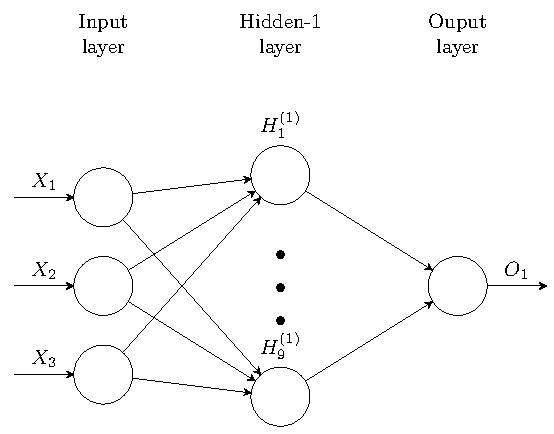
\includegraphics{nnet.pdf}

\subsection{Data}

	The neural network takes 3 inputs, where the design matrix $\mathbf{X}$ is $N \times 3$ ; however, this can be generalized to any number of $M$ inputs for a  $N \times M$ design matrix. The neural network is then fed one observation at a time, $\mathbf{x}^\intercal_i$ for $i = 1, 2, ..., N$
	
	$$
	\mathbf{X} = \begin{bmatrix}
	x_{11} & x_{12} & x_{13} \\
	x_{21} & x_{22} & x_{23} \\
	 & \cdots & \\
	x_{N1} & x_{N2} & x_{N3} \\
	\end{bmatrix} = 
	\begin{bmatrix}
	\mathbf{x}^\intercal_1 \\
	\mathbf{x}^\intercal_2 \\
	 \cdots \\
	\mathbf{x}^\intercal_N \\
	\end{bmatrix}
	$$

	There is one output target 
	$$
	\mathbf{y} = \begin{bmatrix}
	y_1 \\
	y_2 \\
 	 \cdots \\
 	y_N \\
	\end{bmatrix}
	$$
	

\subsection{First Hidden Layer}

	In the first hidden layer there are 9 hidden units $H^{(1)}_1, H^{(1)}_2, ..., H^{(1)}_9$. Each hidden unit sees each of the three 3 inputs, aggregates the inputs with weights and passes that hidden output to an activation function. The activation function used in the first hidden layer is logistic,
	
	$$
	H^{(1)}_k = f(z) = \frac{1}{1 + e^{-z}}
	$$
	
	where $z = w^{(1)}_1 x_i1 + w^{(1)}_2 x_i2 + w^{(1)}_3 x_i3$.
	
	For each hidden unit, we have three weights $\mathbf{w}^{(1)}$

\subsection{Second Hidden Layer}

	In the second hidden layer there is 1 hidden units (the output unit). Because there is only one output, $y_i$, there is only the need for one hidden unit. 
	
	The second hidden layer expects 9 inputs from the first hidden layer. The activation function is simply the identity function $g(z) = z$, where $z = w^{(2)}_1 x_i1 + w^{(2)}_2 x_i2 + w^{(2)}_9 x_i3$.
	
	
	
\section{Feed Forward}

For each observation $i$, we take input $\mathbf{x}^\intercal_i$ and pass it to the first layer.

	$$
	\mathbf{x}^\intercal_i \mathbf{w}^{(1)}
	$$
	








\end{document}